\documentclass[10pt]{article}



\usepackage{sectsty}
\chapternumberfont{\Large}
\chaptertitlefont{\Large}
\usepackage{graphicx}
\usepackage{eso-pic}
\usepackage{subfigure}
\usepackage{booktabs}% http://ctan.org/pkg/booktabs
\newcommand{\tabitem}{~~\llap{\textbullet}~~}
\usepackage[english]{babel}
\usepackage[utf8]{inputenc}
\usepackage[T1]{fontenc}
\usepackage{fancyhdr}
\usepackage{float}
\usepackage[justification=centering]{subfig}
\usepackage[margin = 0.8in]{geometry}
\usepackage{titlesec} % Control title sizes
\usepackage{multirow}
\usepackage{mathtools}
\usepackage{setspace}
\usepackage{wrapfig}
\usepackage{yfonts}
\usepackage{url}
\usepackage{placeins}
\usepackage{amsmath}
\usepackage{amssymb}
\DeclareMathOperator{\Tr}{Tr}
\usepackage{gensymb}
\usepackage{emptypage}
\usepackage{lastpage}
\usepackage[colorlinks = true, linkcolor = blue]{hyperref}
\numberwithin{equation}{section}
\numberwithin{figure}{section}
\numberwithin{table}{section}
\usepackage{wrapfig}
\usepackage{tikz} % For drawing figures
\usepackage{verbatim} % Making comment section
\usepackage{dirtytalk}
\usepackage{caption}
\usepackage{subcaption}
\usepackage{indentfirst}

\begin{titlepage}
\thispagestyle{empty}
\end{titlepage}

\begin{document}



\begin{center}
%\includegraphics[scale=0.5]{fig/windmill.PNG}

\includegraphics[height=4cm]{Figures/dtulogo.jpg}
\end{center}

\begin{center}
\vspace*{1.8cm}
\newcommand{\HRule}{\rule{\textwidth}{1mm}}
\HRule\\
[0cm]\fontsize{14}{16}{\textbf{Machine Learning and Data Mining Report 2 \linebreak Algerian Forest Fires}} \linebreak 
\fontsize{16}{32}{\textbf{\\[10pt] }}
\HRule\\[0.5cm]
\renewcommand{\arraystretch}{1}

\vspace*{0.5cm}
\Large
\vspace*{0.5cm}


\begin{tabular}{l l l l}
\large{Student no.:{\ \ s192322\ }} & \large{Student:{\ \ Paolo Dalpasso\ \ \ \ \ \ \ \ \ }}\\
\large{Student no.:{\ \ s206063\ }} & \large{Student:{\ \ Changzhi Ai\ \ \ \ \ \ \ \ \ }}\\
\large{Student no.:{\ \ s192624\ }} & \large{Student:{\ \ Boris Guillerey\ \ \ \ \ \ \ \ \ }}\\
\vspace{1cm}
\end{tabular}\\ 

\end{center}

\setlength{\parindent}{5ex}

\pagebreak

\clearpage
\setcounter{page}{1}
\tableofcontents

\pagebreak

% \section*{Contributions}
%  The group split the work amongst themselves as is depicted in \autoref{table:contributions}.

% \begin{table}[H]
% \centering
% \begin{tabular}{l|l|l|l|}
% \cline{2-4}
%                                                                                           & \textbf{Changzhi} & \textbf{Paolo} & \textbf{Boris} \\ \hline
% \multicolumn{1}{|l|}{Introduction}                                                        &    X               &     X           &     X           \\ \hline
% \multicolumn{1}{|l|}{Regression part A}                                                   &    X               &      X          &      X          \\ \hline
% \multicolumn{1}{|l|}{Regression part B}                                                   &    X               &      X          &      X          \\ \hline
% \multicolumn{1}{|l|}{Results of the double cross validation}                              &    X               &       X         &      X          \\ \hline
% \multicolumn{1}{|l|}{Comparison of three models: statistical evaluation}                  &                   &        X        &                \\ \hline
% \multicolumn{1}{|l|}{Classification}                                                      &                   &         X       &                \\ \hline
% \multicolumn{1}{|l|}{Comparison with existing works}                                      &                   &                &     X           \\ \hline
% \multicolumn{1}{|l|}{Comparison of three models: statistical evaluation (classification)} &                   &          X      &                \\ \hline
% \multicolumn{1}{|l|}{Summary}                                                             &    X           &                &                \\ \hline
% \end{tabular}
% \caption{Contribution table}
% \label{table:contributions}
% \end{table}                                                          

\section{Introduction}
Project report 2 naturally follows project report 1 on "Algerian Forest Fires prediction". The FWI (Fire Weather Index) indicates the potential intensity of a wild fire and it's calculated integrating the BUI and ISI indexes, which are obtained from the fire weather observations and fuel moisture code, as shown in FIG. \ref{FWI}. Thus, we will choose FWI attribute as a prediction object in the whole project 2.

\begin{figure}[H]
    \centering
    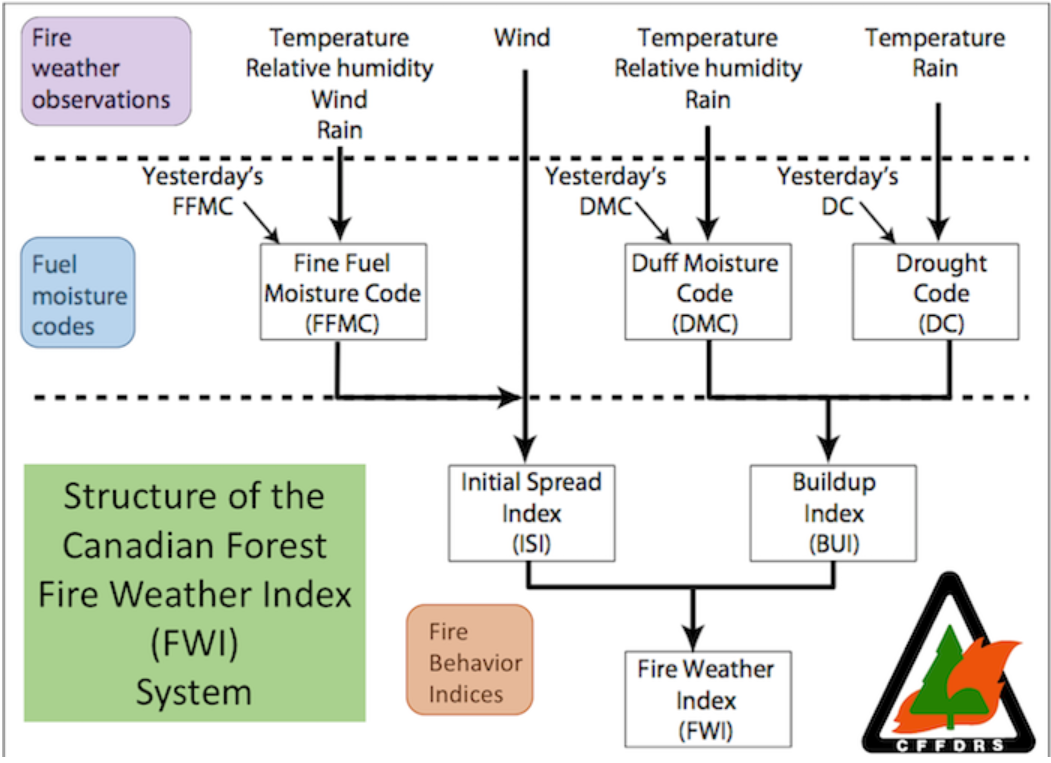
\includegraphics[scale = 0.5]{Figures/Fire_weather_index.png}
    \caption{FWI calculation}
    \label{FWI}
\end{figure}


\section{Regression part A}
\subsection{Objective of the regression}
The aim of our study is to predict the Fire Weather Index (FWI) for the 2 different regions Bejaia and Sidi-Bel-Abbes.  Both regions were monitored for 4 months and meteorological data (Temperature, RH, Ws, Rain) were collected and used to determine other parameters from the Fire Weather Index system (FFMC, DMC, DC, ISI, BUI, FWI), which describes the probability for a wild fire to appear and its intensity.
In the article, from which we took inspiration for the report, it's stated that the rain attribute was not considered to train the machine learning algorithm.
On the contrary in this report, the FWI index will be first predicted only using meteorological data to test if these are enough to give an acceptable prediction of the FWI.

%All attributes are firstly normalized with mean 0 and standard deviation 1.

\subsection{Regularization}

The FWI is predicted using a linear model, in which a regularization factor $\lambda$ is introduced to improve the model performance.

The cost function could be calculated and this objective can be solved by computing the derivative and setting it equal to zero. Then the optimal weights $\omega^*$ as a function of $\lambda$ could be obtained as follows:
\begin{equation*}
    E_{\lambda}(w,w_0) = {\parallel y - w_0 - \hat{X}w \parallel}^2 + \lambda w^2
\end{equation*}
\begin{equation*}
    {\omega^*} = \frac{\hat{X}^T \hat{y}}{\hat{X}^T \hat{X} + {\lambda}I}
\end{equation*}
$\lambda$ controls the complexity of model. Changing $\lambda$, variance/bias ratio of the model would be tuned. Therefore low $\lambda$, corresponds to models with high variance and low bias, while high $\lambda$, corresponds to models with low variance and high bias.
The model is tested on a range of $\lambda$ and the optimal one, which gives the lowest generalized error can be selected.

The plots of the training and test error of the models trained only with the 4 meteorological attributes and with all the attributes are shown in Fig.\ref{regressA_comp}.

\begin{figure}[H]
    \centering
    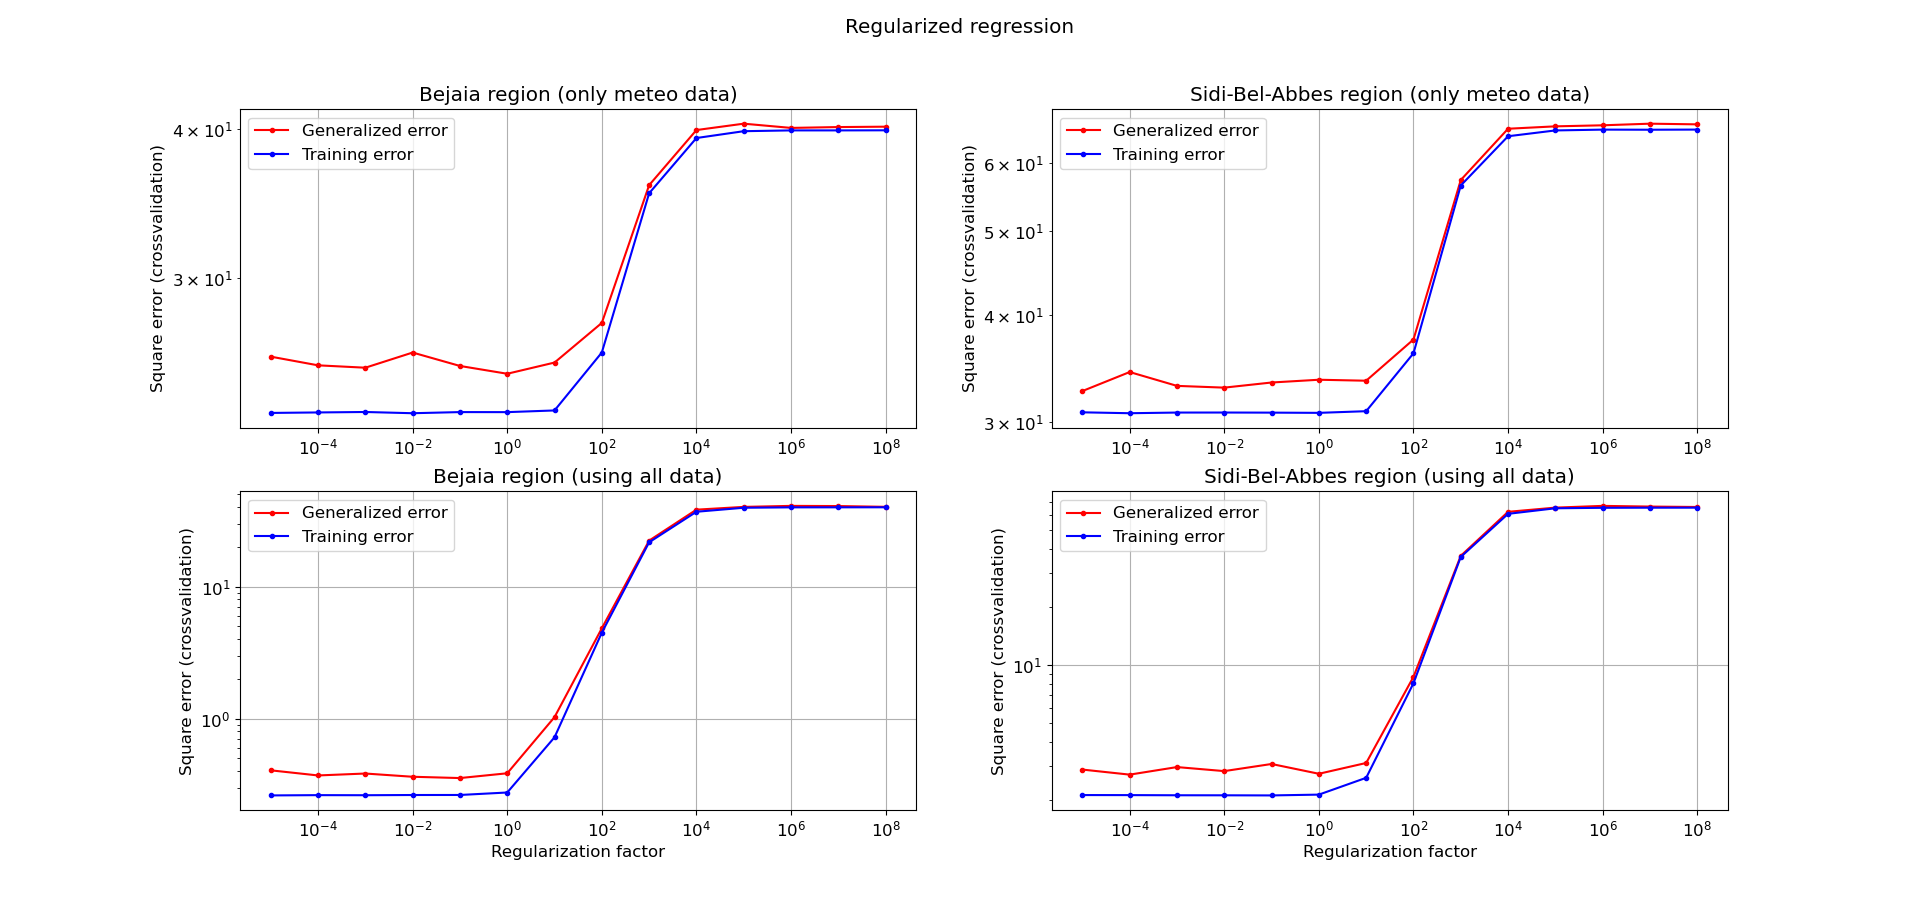
\includegraphics[scale = 0.4]{Figures/regressionA_comparison_with_without_all_data_both_regions.png}
    \caption{Training error and generalized error for regularized regression for both regions}
    \label{regressA_comp}
\end{figure}
As shown in \ref{regressA_comp} the generalization error is drastically lower when considering all the attributes and not only the meteorological data. For the Bejaia region the error is 3 times lower, while for the Sidi-Bel-Abbes it is 4 times lower.

Therefore, even if it was stated in the previous report, that the regression prediction would have been based only on the meteorological data, to obtain an acceptable prediction of FWI, it is clear that it is necessary to consider all the attributes of the dataset according to these results. 

Furthermore, the optimal value of the regularization factor is not clearly identified from the graphs, although it can be said that it is located in all the cases in a range from $10^{-5}$ to $10$. The double cross validation applied later on, will give a better assessment of this value. Finally, we also assess the effect of including quadratic terms in the observation matrix. The reduction of the generalization error is observed on \autoref{fig:quadratic} and for this case an optimal value of $\lambda = 10$ could be determined.

\begin{figure}[H]
    \centering
    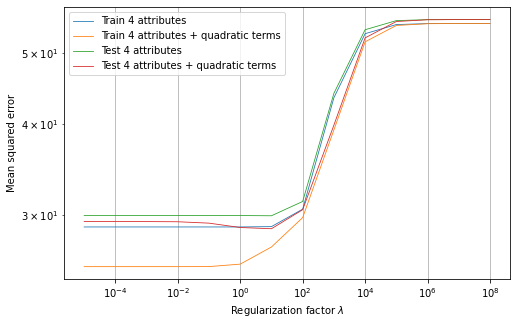
\includegraphics[scale=0.5]{Figures/RegularizationFactor_Meteo.png}
    \caption{Squared error as a function of regularization factor lambda for both regions when applying first four attributes as data matrix X and effect of adding quadratic terms.}
    \label{fig:quadratic}
\end{figure}

% \begin{figure}[H]
%    \centering
%    \includegraphics[sc%ale=0.4]{Figures/linear%_regression_part_a.png}
%    \caption{Mean %coefficient values as a %function of regularization factor lambda and squared error as a function of regularization factor lambda for both region.}
%    \label{fig:lr}
%\end{figure}

\subsection{Effects of the attributes}

The effect of the attributes in the linear regression can be assessed by representing the variation of their weights with the regularization factor. \autoref{fig:Weights} depicts this variation if considering only the meteorological data. In this case, it appears as expected that the temperature and wind speed affect positively the FWI while the rain and relative humidity affect it negatively. On the other hand, if considering the 9 attributes, the results is mostly influenced positively by the ISI, BUI indices, which makes perfectly sense when considering the construction of the FWI index as presented in \autoref{FWI}.

\begin{figure}[H]
    \centering
    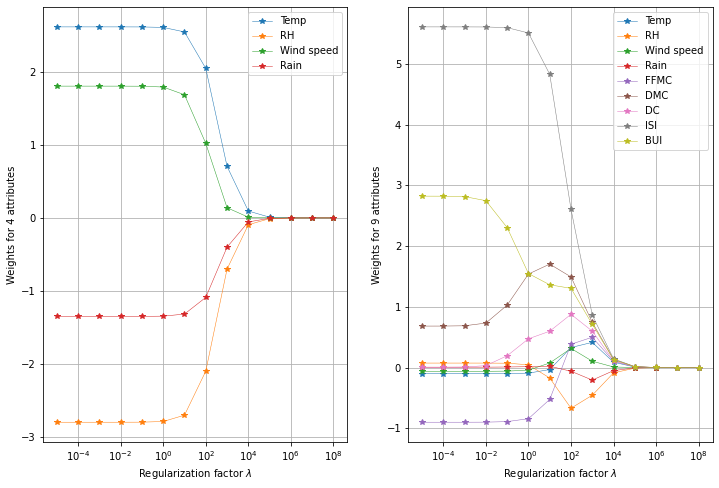
\includegraphics[scale=0.6]{Figures/Weights.png}
    \caption{Mean coefficient values as a function of regularization factor lambda using data from both regions as inputs.}
    \label{fig:Weights}
\end{figure}

%\subsection{Difference between regions}
%Difference between two regions are also studied. It is obvious that the errors of Bajaia region is lower that that of Sidi region.
%\begin{figure}[H]
%    \centering
%    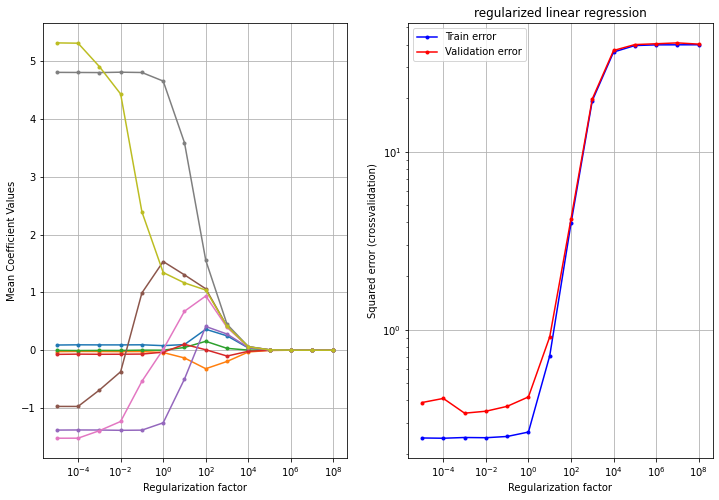
\includegraphics[scale=0.4]{Figures/linear_regression_part_a_Bejaia.png}
%    \caption{Mean coefficient values as a function of regularization factor lambda and squared error as a function of regularization factor lambda for Bejaia region.}
%    \label{fig:lr_Bejaia}
%\end{figure}
%\begin{figure}[H]
%    \centering
%    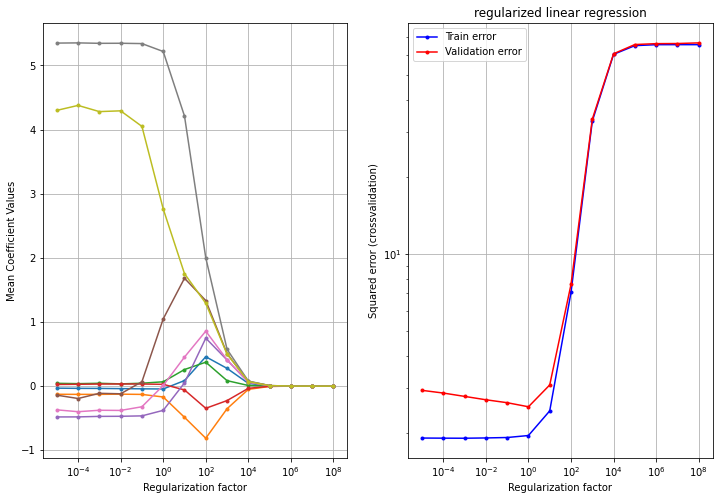
\includegraphics[scale=0.4]{Figures/linear_regression_part_a_Sidi.png}
%    \caption{Mean coefficient values as a function of regularization factor lambda and squared error as a function of regularization factor lambda for Sidi region.}
%    \label{fig:lr_Sidi}
%\end{figure}


%\subsection{Effect of the attributes selection}
%\begin{figure}[H]
%    \centering
%    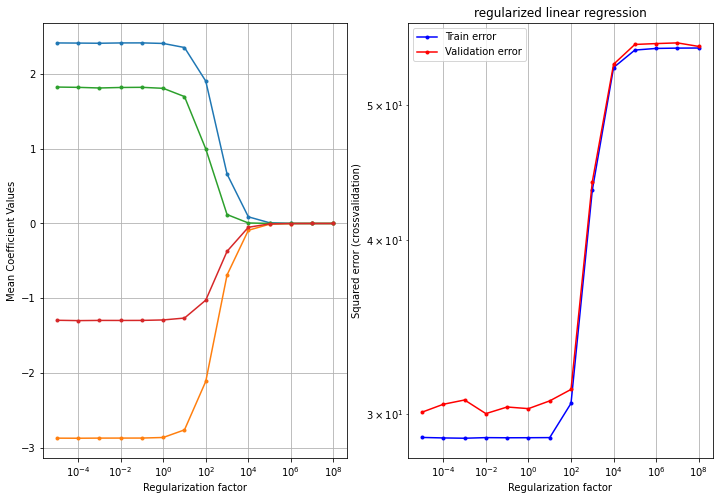
\includegraphics[scale=0.4]{Figures/linear_regression_part_a_4_attributes.png}
%    \caption{Mean coefficient values as a function of regularization factor lambda and squared error as a function of regularization factor lambda for both region when applying first four attributes as data matrix X.}
%    \label{fig:map}
%\end{figure}

\section{Regression part B}

In this section, the FWI is predicted using 3 different models: a regularized linear regression, an Artificial Neural Network (ANN) and a baseline model, which is used as a comparative reference for the other 2 models.
The baseline model consists in a linear regression model with no
features, i.e. it computes the mean of y on the training data, and use this value as prediction for the test set.
A two-layer cross validation (K1 = 10, K2 = 10) is applied to both linear regression and ANN, where each train set of the outer cross validation is splitted in another pair of train and test set, which are used to find the optimal complexity-controlling parameters for both models: respectively $\lambda$ and the number of hidden units \textit{h}, for the regularized linear regression and for the ANN.

After a few tests to determine first approximations of optimal values of $\lambda$ and \textit{h}, the following range were chosen for the inner loop in double cross validation:
\begin{equation*}
\begin{multlined*}

    

    \lambda = [10^{-5}; 10^{9}], \hspace{5pt} multiples \hspace{3pt} of \hspace{3pt} 10 \\
   
    \textit{h} = [1; 10]

\end{multlined*}
\end{equation*}

In the following part, the results are presented when training the models on both regions together, and by separating them. As we see in the previous part, it is indeed expected that the construction of the models differ for the two regions because of the variability of their climate and vegetation. Before applying the double cross validation with 10 inner folds and 10 outer folds, we also discarded one again using only the 4 meteorological attributes to determine FWI. As seen in \autoref{fig:fit}, realized for a simple 2 fold cross validation, the results obtained with only 4 attributes are not satisfactory, as the representation of the estimation versus the true values diverges strongly from the linear line $y=x$.  

\begin{figure}[H]
    \centering
    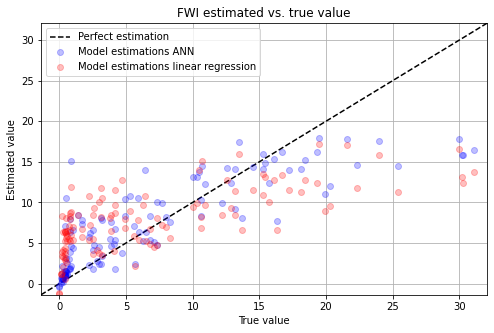
\includegraphics[scale=0.6]{Figures/Est_vs_True_meteo_2fold.png}
    \caption{Comparison of fitted values with true values for ANN and regularized linear regression considering only meteorological attributes (2 fold cross-validation only.}
    \label{fig:fit}
\end{figure}

\subsection{Results of the double cross-validation study}


\subsubsection{Both regions}

Applying the double cross validation to the whole data set gives the results depicted in \autoref{bothregions}. From this study, we observe that the optimal number of hidden units vary significantly for each test set. The error which is in this case the mean squared error, is considerably lower for ANN and linear regression than for the baseline, which indicates the models behave properly. We also notice that $\lambda_i*$ varies in a wide range of values, which is consistent with the results of the linear regression part where we showed that the optimal value of $\lambda$ was not clearly defined when using 9 attributes and no quadratic terms. Finally, we observe that the errors of the ANN are lower than the ones of the linear regression with exception of the third fold. The difference between models will be further assessed in the next part about statistical comparison.


\begin{table}[H]
\centering
\begin{tabular}{l|l|l|l|l|l|ll}
\cline{2-6}
                         & \multicolumn{2}{l|}{\textbf{ANN}} & \multicolumn{2}{l|}{\textbf{Linear regression}} & \textbf{Baseline} &  &  \\ \cline{1-6}
\multicolumn{1}{|l|}{\textbf{Fold}}  & \textbf{$h_i*$} & \textbf{$E_i^{test}$} & \textbf{$\lambda_i*$}  & \textbf{$E_i^{test}$}  & \textbf{$E_i^{test}$} &  &  \\ \cline{1-6}
\multicolumn{1}{|c|}{1}  & 4        & 0.12     & 1                  & 1.08          & 47.81 &  &  \\ \cline{1-6}
\multicolumn{1}{|c|}{2}  & 7        & 0.32      & 1.e-05           & 0.44          & 46.85 &  &  \\ \cline{1-6}
\multicolumn{1}{|c|}{3}  & 4        & 0.55      & 1.e-05           & 0.34          & 68.96  &  &  \\ \cline{1-6}
\multicolumn{1}{|c|}{4}  & 4        & 0.08      & 0.1                & 0.58          & 41.61  &  &  \\ \cline{1-6}
\multicolumn{1}{|c|}{5}  & 4        & 0.74      & 1.e-05           & 1.22          & 58.55 &  &  \\ \cline{1-6}
\multicolumn{1}{|c|}{6}  & 7        & 0.09      & 0.1                & 0.41         & 63.01 &  &  \\ \cline{1-6}
\multicolumn{1}{|c|}{7}  & 9        & 1.30      & 1.e-05           & 1.45          & 72.94  &  &  \\ \cline{1-6}
\multicolumn{1}{|c|}{8}  & 4        & 0.56      & 1                  & 0.96          & 25.49 &  &  \\ \cline{1-6}
\multicolumn{1}{|c|}{9}  & 10       & 0.07      & 1.e-05           & 0.59          & 39.27  &  &  \\ \cline{1-6}
\multicolumn{1}{|c|}{10} & 5        & 8.97      & 1                  & 9.34          & 69.93 &  &  \\ \cline{1-6}
\end{tabular}
\caption{Results of the double cross validation applied to the whole data set (both regions).}
\label{bothregions}
\end{table}



\subsubsection{Regions separately}

As described before, we expect better results when applying the models to the regions separately. \autoref{BejaiaCross} and \autoref{SidiCross} present the results of the double cross validation for both regions. We notice that the optimal $\lambda$ is constantly higher for the Sidi-Bel-Abbès region, which confirms that the model should behave differently on the two regions. We also notice higher errors for the Sidi-Bel-Abbès region which is also associated with a higher variance of the data, as can be seen with the baseline error.

\begin{table}[H]
\centering
\begin{tabular}{c|c|c|c|c|c|}
\cline{2-6}
\multicolumn{1}{l|}{\textbf{}}      & \multicolumn{2}{c|}{\textbf{ANN}}       & \multicolumn{2}{c|}{\textbf{Linear regression}} & \textbf{Baseline}     \\ \hline
\multicolumn{1}{|c|}{\textbf{Fold}} & \textbf{$h_i*$} & \textbf{$E_i^{test}$} & \textbf{$\lambda_i*$}  & \textbf{$E_i^{test}$}  & \textbf{$E_i^{test}$} \\ \hline
\multicolumn{1}{|c|}{1}             & 7               & 0.41                  & 1e-05                     & 0.42                   & 20.4                  \\ \hline
\multicolumn{1}{|c|}{2}             & 9               & 0.07                   & 1e-05                   & 0.108                   & 21.42                  \\ \hline
\multicolumn{1}{|c|}{3}             & 3               & 0.04                  & 1e-05                     & 0.12                     & 26.98                  \\ \hline
\multicolumn{1}{|c|}{4}             & 7               & 0.24                  & 1e-05                  & 1.11                     & 18.33                  \\ \hline
\multicolumn{1}{|c|}{5}             & 5               & 0.51                  & 1e-05                    & 0.39                   & 40.77                  \\ \hline
\multicolumn{1}{|c|}{6}             & 9               & 0.03                  & 1e-05                    & 0.13                   & 15.63                  \\ \hline
\multicolumn{1}{|c|}{7}             & 7               & 2.45                  & 1e-05                    & 0.52                   & 156.45                  \\ \hline
\multicolumn{1}{|c|}{8}             & 8               & 6.23                  & 1e-05                    & 2.29                   & 93.84                  \\ \hline
\multicolumn{1}{|c|}{9}             & 5               & 0.05                  & 1e-05                    & 0.55                   & 27.48                  \\ \hline
\multicolumn{1}{|c|}{10}             & 3               & 0.02                  & 1e-05                    & 0.15                   & 19.02                  \\ \hline
\end{tabular}
\caption{Bejaia region}
\label{BejaiaCross}
\end{table}


\begin{table}[H]
\centering
\begin{tabular}{c|c|c|c|c|c|}
\cline{2-6}
\multicolumn{1}{l|}{\textbf{}}      & \multicolumn{2}{c|}{\textbf{ANN}}       & \multicolumn{2}{c|}{\textbf{Linear regression}} & \textbf{Baseline}     \\ \hline
\multicolumn{1}{|c|}{\textbf{Fold}} & \textbf{$h_i*$} & \textbf{$E_i^{test}$} & \textbf{$\lambda_i*$}  & \textbf{$E_i^{test}$}  & \textbf{$E_i^{test}$} \\ \hline
\multicolumn{1}{|c|}{1}             & 5               & 1.024                 & 1                    & 0.59                  & 51.58                  \\ \hline
\multicolumn{1}{|c|}{2}             & 4               & 1.49                   & 1                   & 0.29                   & 56.27                  \\ \hline
\multicolumn{1}{|c|}{3}             & 4               & 0.19                 & 1                     & 0.23                     & 26.98                  \\ \hline
\multicolumn{1}{|c|}{4}             & 3               & 0.13                  & 1                   & 0.11                     & 24.28                  \\ \hline
\multicolumn{1}{|c|}{5}             & 8               & 1.68                  & 1                    & 1.55                  & 93.70                  \\ \hline

\multicolumn{1}{|c|}{6}             & 7               & 20.45                  & 0.1                    & 24.19                   & 65.63                  \\ \hline

\multicolumn{1}{|c|}{7}             & 2               & 13.61                  & 1                    & 3.2                   & 176.02                  \\ \hline

\multicolumn{1}{|c|}{8}             & 3               & 2.77                  & 1                    & 4.5                   & 111.05                  \\ \hline

\multicolumn{1}{|c|}{9}             & 3               & 0.72                  & 1                    & 0.39                   & 40.54                  \\ \hline

\multicolumn{1}{|c|}{10}             & 7               & 0.58                  & 1                    & 2.77                   & 54.96                  \\ \hline
\end{tabular}
\caption{Sidi-Bel-Abbes region}
\label{SidiCross}
\end{table}


\subsection{Comparison of three models: statistical evaluation}

The performance among the 3 models is compared statistically, using Setup I, which uses a t-test with $\alpha = 0.05$ and H$_0: \theta = \theta_A - \theta_B $, where $\theta_A$ and $\theta_B$ are the performances, i.e. test error, for model A and model B.\\

The results for the 2 regions are shown, respectively in Table \ref{Table1} and Table \ref{Table2}. 

\subsubsection{9 attributes case}

The statistical comparison among the 3 models is similar for both regions as can be seen in the tables below.
The comparison between the regularized linear regression and the baseline shows a negative confident interval, indicating that the baseline has an higher test error and the very low p-value, confirms that this result is not due to chance. 
Therefore, it can be concluded that the regularized regression is a better model than the baseline one.
The same conclusion, can be drawn regarding the comparison between the ANN and the baseline. Also in this case the CI is negative and low p-value allows to conclude, with a nice margin of certainty, that the ANN model has a better performance than the baseline one.

The comparison between the ANN model and the regularized linear regression model shows a CI around 0, which indicates that the 2 models have a similar performance. Furthermore, the relatively high p-value indicates that there is no effect, i.e. the hypothesis $M_A = M_B$ can not be discarded. Therefore, there is not enough evidence to conclude that the ANN model is better than the linear regression one or the other way around.

\begin{table}[H]
\centering
\begin{tabular}{|c|c|c|c|c|} \hline
\textbf{Model A}  & \textbf{Model B}  & \textbf{$\theta_L$} & \textbf{$\theta_U$} & \textbf{p-value} \\ \hline
Regularized regression & Baseline          & -5.54               & -4.16               & 2.4$e^{-27}$     \\ \hline
ANN               & Baseline          & -5.47               & -4.25              & 1.8$e^{-31}$     \\ \hline
ANN               & Regularized regression & -0.16              & 0.14               & 0.43008    \\ \hline
\end{tabular}
\caption{Confidence intervals and p-values for the pairwise models in Bejaia region}
\label{Table1}
\end{table}


\begin{table}[H]
\centering
\begin{tabular}{|c|c|c|c|c|} \hline
\textbf{Model A}  & \textbf{Model B}  & \textbf{$\theta_L$} & \textbf{$\theta_U$} & \textbf{p-value} \\ \hline
Regularized regression & Baseline          & -6.82               & -5.14              & 1.4$e^{-27}$     \\ \hline
ANN               & Baseline          & -6.73               & -5.26           & 2.28$e^{-32}$     \\ \hline
ANN               & Regularized regression & -0.24             & 0.20              & 0.4331   \\ \hline
\end{tabular}
\caption{Confidence intervals and p-values for the pairwise models in Sidi-Bel-Abbes region}
\label{Table2}
\end{table}








\subsubsection{4 attributes case}

For comparison, the statistical assessment was also realized for models trained on only meteorological attributes (this time for both regions together). The main difference in this case was that the ANN gives significantly better results than the linear regression, as can be seen in \autoref{statisticMeteo}, where the p-value associated with this comparison is significantly low. This is expected as when considering the 9 attributes, it exists a direct relationship between between the FWI indices and the final FWI index, which is well captured by a linear regression. To the contrary, when considering only the meteorological attributes, the linear regression failed to predict satisfactorily the FWI index whereas the ANN helps significantly to capture the structure of the data.

\begin{table}[H]
\centering
\begin{tabular}{|c|c|c|c|c|} \hline
\textbf{Model A}  & \textbf{Model B}  & \textbf{$\theta_L$} & \textbf{$\theta_U$} & \textbf{p-value} \\ \hline
Regularized regression & Baseline          & -31.9               & -16.9              & 3.4$e^{-10}$     \\ \hline
ANN               & Baseline          & -48.9               & -29.6           & 2.0$e^{-14}$     \\ \hline
ANN               & Regularized regression & -19.1             & -10.7              & 1.0$e^{-11}$   \\ \hline
\end{tabular}
\label{porcodio2}
\caption{Confidence intervals and p-values for the pairwise models for the whole data set but considering only the 4 meteorological attributes.}
\label{statisticMeteo}
\end{table}





\section{Classification}
In this section 3 different models are used to predict the Fire/not fire class.
For this task, a Logistic regression, a K-nearest neighbors and a baseline model are implemented and statistically compared.

As for the Logistic regression, a 2-layer cross validation (K1 = 10, K2 = 10) is used to obtain the optimal lambda for each training set, i.e. the lambda that gives the lowest test error for each training set.
Likewise, a 2-layer cross validation is applied to the KNN model and the inner cross validation is used to find the ideal number of k neighbours, which gives the lowest test error for each training set.
A simple model, which compute the largest class on the training
data, and predict everything in the test-data as belonging to that class is used as baseline model.
The results of the classification is shown in Table \ref{Table11} and Table \ref{Table22}

\begin{table}[H]
\centering
\begin{tabular}{c|c|c|c|c|c|}
\cline{2-6}
\multicolumn{1}{l|}{\textbf{}}      & \multicolumn{2}{c|}{\textbf{KNN}}       & \multicolumn{2}{c|}{\textbf{Logistic regression}} & \textbf{Baseline}     \\ \hline
\multicolumn{1}{|c|}{\textbf{Fold}} & \textbf{$k_i*$} & \textbf{$E_i^{test}$} & \textbf{$\lambda_i*$}  & \textbf{$E_i^{test}$}  & \textbf{$E_i^{test}$} \\ \hline
\multicolumn{1}{|c|}{1}             & 7               & 0.076                  & 1e-08                     & 0                & 0.38                  \\ \hline
\multicolumn{1}{|c|}{2}             & 4               & 0.153                   & 1.75e-06                     & 0                   & 0.38                  \\ \hline
\multicolumn{1}{|c|}{3}             & 5               & 0.166                  & 1e-08                     & 0                     & 0.5                  \\ \hline
\multicolumn{1}{|c|}{4}             & 10               & 0.166                  & 2.94e-06                     & 0.083                     & 0.66                  \\ \hline
\multicolumn{1}{|c|}{5}             & 4               & 0                  & 7.9e-08                     & 0                   & 0.66                  \\ \hline
\multicolumn{1}{|c|}{6}             & 8               & 0.083                  &  6.25e-07                     & 0                   & 0.66                  \\ \hline
\multicolumn{1}{|c|}{7}             & 8             & 0                   & 1e-08                     & 0.083                   & 1                  \\ \hline
\multicolumn{1}{|c|}{8}             & 6               & 0.166                  & 1e-08                     & 0.083                   & 0.41                  \\ \hline
\multicolumn{1}{|c|}{9}             & 4               & 0                   & 1.04e-06                     & 0                  & 0.83                  \\ \hline
\multicolumn{1}{|c|}{10}            & 4               & 0.083                  & 1e-08                     &   0                 & 0.66                  \\ \hline
\end{tabular}
\caption{Bajaia region}
\label{Table11}
\end{table}


\begin{table}[H]
\centering
\begin{tabular}{c|c|c|c|c|c|}
\cline{2-6}
\multicolumn{1}{l|}{\textbf{}}      & \multicolumn{2}{c|}{\textbf{KNN}}       & \multicolumn{2}{c|}{\textbf{Logistic regression}} & \textbf{Baseline}     \\ \hline
\multicolumn{1}{|c|}{\textbf{Fold}} & \textbf{$k_i*$} & \textbf{$E_i^{test}$} & \textbf{$\lambda_i*$}  & \textbf{$E_i^{test}$}  & \textbf{$E_i^{test}$} \\ \hline
\multicolumn{1}{|c|}{1}             & 1               & 0.15                  & 0.03                     & 0                & 0.61                  \\ \hline
\multicolumn{1}{|c|}{2}             & 3               & 0                   & 0.15                     & 0                   & 0.69                  \\ \hline
\multicolumn{1}{|c|}{3}             & 3               & 0.083                 & 1e-08                     & 0                     & 016                  \\ \hline
\multicolumn{1}{|c|}{4}             & 3               & 0.083                  & 8.28e-06                     & 0                     & 0.16                  \\ \hline
\multicolumn{1}{|c|}{5}             & 3               & 0.41                  & 3.9e-05                     & 0                   & 0.41                  \\ \hline
\multicolumn{1}{|c|}{6}             & 3               & 0                  &  1e-08                     & 0                   & 0.16                  \\ \hline
\multicolumn{1}{|c|}{7}             & 9             & 0                   & 1e-08                     & 0.083                   & 0                  \\ \hline
\multicolumn{1}{|c|}{8}             & 3               & 0.083                  & 2.8e-08                     & 0.083                   & 0.5                  \\ \hline
\multicolumn{1}{|c|}{9}             & 6               & 0.33                   & 0.004                     & 0                  & 0.16                  \\ \hline
\multicolumn{1}{|c|}{10}            & 3               & 0.16                  & 2.94e-06                     &   0                 & 0.58                  \\ \hline
\end{tabular}
\caption{Sidi-Bel-Abbes region}
\label{Table22}
\end{table}

Both KNN model and the Logistic regression predict very accurately the fire/not fire class in both region, respectively with an error of 0.0893 and 0.083 for the Bejaia region and 0.1299 and 0.083 for the Sidi-Bel-Abbes region.



\subsection{Comparison with existing works}

Existing works have already been performed on the same data set. Especially, \cite{article} presents the results of different works when using a regression tree. We therefore also implemented a regression tree to fit our data. The results are summarized in \autoref{existingWorks} where we notice that the accuracy is in every case close to 80\%. Here it is worth noticing that those results are considered based on the meteorological attributes, which explains the relative low accuracy of those models. In our study, we chose to focus more in the case where all the attributes are known. This would be the case if applying the FWI system method described in \cite{FWI_Wagner} to determine the FWI indices from the knowledge of the 4 meteorological attributes.

\begin{table}[H]
\centering
\begin{tabular}{|c|c|}
\hline
\textbf{Reference} & \textbf{Accuracy (\%)} \\ \hline
F.Abid             & 82.9                   \\ \hline
Stojanova          & 81.2                   \\ \hline
This work          & 80.7                   \\ \hline
\end{tabular}
\caption{Comparison of results for simple decision trees applied to predict the FWI index from the 4 meteorological attributes.}
\label{existingWorks}
\end{table}






\subsection{Comparison of three models: statistical evaluation}
The three models are statistically compared using Setup I, which consists in using the Mcnemar test to compare the performances between 2 models at the time.





\begin{table}[H]
\centering
\begin{tabular}{|c|c|c|c|c|} \hline
\textbf{Model A}  & \textbf{Model B}  & \textbf{$\theta_L$} & \textbf{$\theta_U$} & \textbf{p-value} \\ \hline
Logistic regression & Baseline          & -0.56               & -0.36            & 1.4$e^{-13}$     \\ \hline
KNN               & Baseline          & -0.6               & -0.47             & 1.7$e^{-16}$     \\ \hline
Logistic regression   & KNN & -0.039            & 0.0391           & 0.13    \\ \hline
\end{tabular}
\caption{Confidence intervals and p-values for the pairwise models in Bejaia region}
\end{table}


\begin{table}[H]
\centering
\begin{tabular}{|c|c|c|c|c|} \hline
\textbf{Model A}  & \textbf{Model B}  & \textbf{$\theta_L$} & \textbf{$\theta_U$} & \textbf{p-value} \\ \hline
Logistic regression & Baseline          & -0.56               & -0.38               & 3.2$e^{-15}$     \\ \hline
KNN               & Baseline          & -0.43               & -0.28              & 2.07$e^{-14}$     \\ \hline
Logistic regression  & KNN & -0.0007            & 0.08           & 0.125    \\ \hline
\end{tabular}
\caption{Confidence intervals and p-values for the pairwise models in Sidi-Bel-Abbes region}
\end{table}

The results are, again, similar for both regions.
Both comparisons between Logistic regression vs. Baseline and KNN model vs. Baseline, show a negative CI, which indicates that the Baseline error is likely higher than the Logistic regression and KNN one. Moreover the low p-value indicates us that this result is not likely due to chance.
Therefore we can conclude that both Logistic regression and KNN have a better performance in predicting the fire/not fire class in both regions.
The comparison between Logistic regression and KNN, gives a CI around 0.
This could indicates that the two models have a very similar performance, if not identical. Nevertheless, the high p-value indicates that such result is likely due to chance, therefore it's not possible to conclude that the Logistic regression model has a better performance than the KNN one.


\section{Summary}
For regression, we used three different models (regularized linear regression, artificial neural network and baseline model) implemented two level cross validation to train and predict FWI attribute. It is obvious that ANN and linear regression models have lower test errors than baseline model. Furthermore, we can see that ANN model is even a little better than linear
regression. Thus, FWI attribute could be well predicted by ANN and linear regression in our case.

For classification, k-nearest neighbor, logistic regression and baseline models were carried out to train and predict fire or not fire attribute. Both KNN and logistic regression show a good performance on predicting fire situation. Especially, logistic regression have a really low test error for fire prediction.

It is worth pointing out that both regions have a very similar fire prediction situation even though there is a larger error for Sidi-Bel-Abbes region. Therefore, those models may be used as a method to predict forest fire. 

\section{Question answers}

\subsection*{Question 1: answer C}

The correct answer can be obtained by considering a separation at $\hat{y}=0$ and then increasing this value. At $\hat{y}=0$, TPR and FPR equal to 1 when all attributes are classified positive. From the point (1,1), on the ROC curve, we see that TPR should decrease to 0.75. When the separation increases, one observation is classified negative, and TPR decreases if this observation is in reality positive. This gives answer A or C. When the separation increases again, if the second observation is again positive (as in prediction A), TPR would decrease to 0.5, which is not the case. The right answer is therefore C.

\subsection*{Question 2: answer D}
The impurity gain is calculated using:
\begin{equation*}
    \Delta = I(r) - \sum_{k = 1}^{K}\frac{N(V_{k})}{N(r)}I(V_k)
\end{equation*}
using the classification error as purity function $I(v) = 1 - max_c p(c|v) $
So we calculate I(r), I(v1), I(v2):

\begin{equation*}
I(r) = 1 - \frac{5}{14} = \frac{9}{14}
\end{equation*}
\begin{equation*}
    I(v1) = 1 - \frac{5}{13} = \frac{8}{13}\\
\end{equation*}
\begin{equation*}
      I(v2) = 1-1 = 0
\end{equation*}

so:
\vspace{10pt}
\begin{equation*}
    \Delta = I(r) - \frac{N(v1)}{N(r)}I(v1) - \frac{N(v2)}{N(r)}I(v2) =
\end{equation*}
\begin{equation*}
    = \frac{9}{14} - \frac{13}{14}\cdot\frac{8}{13} = \frac{1}{14 }= 0,072
\end{equation*}

the solution which is closer to our result is answer D.


\vspace{5mm}

\subsection*{Question 4: answer D}
When b1 $\leq$ -0.76 is false and b2 $\leq$ 0.03 is also false, we can get congestion level 1. If b1 $\leq$ -0.76 is false and b2 $\leq$ 0.03 is true, we could have congestion level 2. Now, we consider the case that b1 $\leq$ -0.76 is true. If b1 $\leq$ -0.16 is true, we have congestion level 4. Otherwise, if b2 $\leq$ 0.01 is true, we also have congestion level 1, or we have congestion level 3. 


\subsection*{Question 5: answer C}

The total time is calculated using the equation:

\begin{equation*}
    5\cdot[(5\cdot4\cdot25 \hspace{2pt} ms) + 25\hspace{2pt} ms + (5\cdot4\cdot9 \hspace{2pt} ms) + 9 \hspace{2pt} ms] = 3570 \hspace{2pt} ms 
\end{equation*}
where $5\cdot [ ]$ indicate the outer cross validation $K_1$ = 5, $5\cdot4$ is the loop which applied to each hidden unit/lambda the inner cross validation $K_2$ = 4, once the best paramter is found, another train/test is done in the outer set for both ANN and regularized regression.

\begin{thebibliography}{}
\bibitem{article} Faroudja Abid, Nouma Izeboudjen, 06 February 2020, \textit{Predicting Forest Fire in Algeria Using Data Mining Techniques: Case Study of the Decision Tree Algorithm}

\bibitem{FWI_Wagner} C.E Van Wagner, 1987, \textit{Development and Structure of the Canadian Forest Fire Weather Index System}

\end{thebibliography}

\end{document}